\documentclass[11pt]{article}
\usepackage{geometry,marginnote} % Pour passer au format A4
\geometry{hmargin=1cm, vmargin=1cm} % 

% Page et encodage
\usepackage[T1]{fontenc} % Use 8-bit encoding that has 256 glyphs
\usepackage[english,french]{babel} % Français et anglais
\usepackage[utf8]{inputenc} 

\usepackage{lmodern,numprint}
\setlength\parindent{0pt}

% Graphiques
\usepackage{graphicx,float,grffile,units}
\usepackage{tikz,pst-eucl,pst-plot,pstricks,pst-node,pstricks-add,pst-fun,pgfplots} 

% Maths et divers
\usepackage{amsmath,amsfonts,amssymb,amsthm,verbatim}
\usepackage{multicol,enumitem,url,eurosym,gensymb,tabularx}

\DeclareUnicodeCharacter{20AC}{\euro}



% Sections
\usepackage{sectsty} % Allows customizing section commands
\allsectionsfont{\centering \normalfont\scshape}

% Tête et pied de page
\usepackage{fancyhdr} \pagestyle{fancyplain} \fancyhead{} \fancyfoot{}

\renewcommand{\headrulewidth}{0pt} % Remove header underlines
\renewcommand{\footrulewidth}{0pt} % Remove footer underlines

\newcommand{\horrule}[1]{\rule{\linewidth}{#1}} % Create horizontal rule command with 1 argument of height

\newcommand{\Pointilles}[1][3]{%
  \multido{}{#1}{\makebox[\linewidth]{\dotfill}\\[\parskip]
}}

\newtheorem{Definition}{Définition}

\usepackage{siunitx}
\sisetup{
    detect-all,
    output-decimal-marker={,},
    group-minimum-digits = 3,
    group-separator={~},
    number-unit-separator={~},
    inter-unit-product={~}
}

\setlength{\columnseprule}{1pt}

\begin{document}

\textbf{Nom, Prénom :} \hspace{8cm} \textbf{Classe :} \hspace{3cm} \textbf{Date :}\\

\begin{center}
  \textit{La normalité est une route pavée : on y marche aisément mais les fleurs n’y poussent pas.}  - \textbf{Vincent Van Gogh}
\end{center}

\subsection*{Restituer les connaissances}

\begin{enumerate}
  \item[1.] Nombres négatifs : \dotfill \\
  \item[2.] Nombres opposés \dotfill \\
\end{enumerate}

\subsection*{Représenter des nombres par des opérations}

\begin{multicols}{2}

  \textit{Écrire le nombre négatif et l'opération correspondante.}

  \begin{enumerate}
    \item[1.] $  -5 = $ \dotfill
    \item[2.] $-130 = $ \dotfill
    \item[3.] $-0,5 = $ \dotfill
    \item[4.] $-\pi = $ \dotfill
    \item[5.] $ -\frac{2}{3} = $ \dotfill
    \item[6.] $0 - 25 = $  \dotfill
    \item[7.] $0 - \SI{0,45}{} = $  \dotfill
    \item[8.] $0 - \SI{54000}{} = $  \dotfill   
  \end{enumerate}
  \columnbreak

  \textit{Écrire l'opposé et l'opération correspondante.}

  \begin{enumerate}
    \item[1.] L'opposé de $6$ est \dots \dots car \dotfill
    \item[2.] L'opposé de $-3$ est \dots \dots car \dotfill
    \item[3.] L'opposé de $\SI{1500}{}$ est \dots \dots car \dotfill
    \item[4.] L'opposé de $\SI{-0,4}{}$ est \dots \dots car \dotfill
    \item[5.] L'opposé de $\pi$ est \dots \dots car \dotfill
    \item[6.] L'opposé de $\dfrac{1}{3}$ est \dots \dots car \dotfill
  \end{enumerate}

\end{multicols}

\subsection*{Comparer}

\textit{Ranger par ordre croissant. Utiliser le symbole $<$.}

\begin{enumerate}
  \item[1.] 0; -2; 4; -6; 8; -10
  \Pointilles[1]   
  \item[2.] 15; -10; \SI{1,2}{} ; \SI{-1,1}{} ; \SI{-1,2}{} , \SI{-1,15}{} 
  \Pointilles[1]   
  \item[3.] -300 ; 250 ; \SI{-40000}{} ; -550 ; 0,6 ; -10
  \Pointilles[1]   
\end{enumerate}

\subsection*{Droite graduée}

\textit{Placer les points sur la droite graduée.}

$A = -3 ; B = 2 ; C = \SI{-2,5}{} ; D = \SI{3,5}{} ; E = \SI{0,5}{}$

\begin{figure}[H]
  \centering
  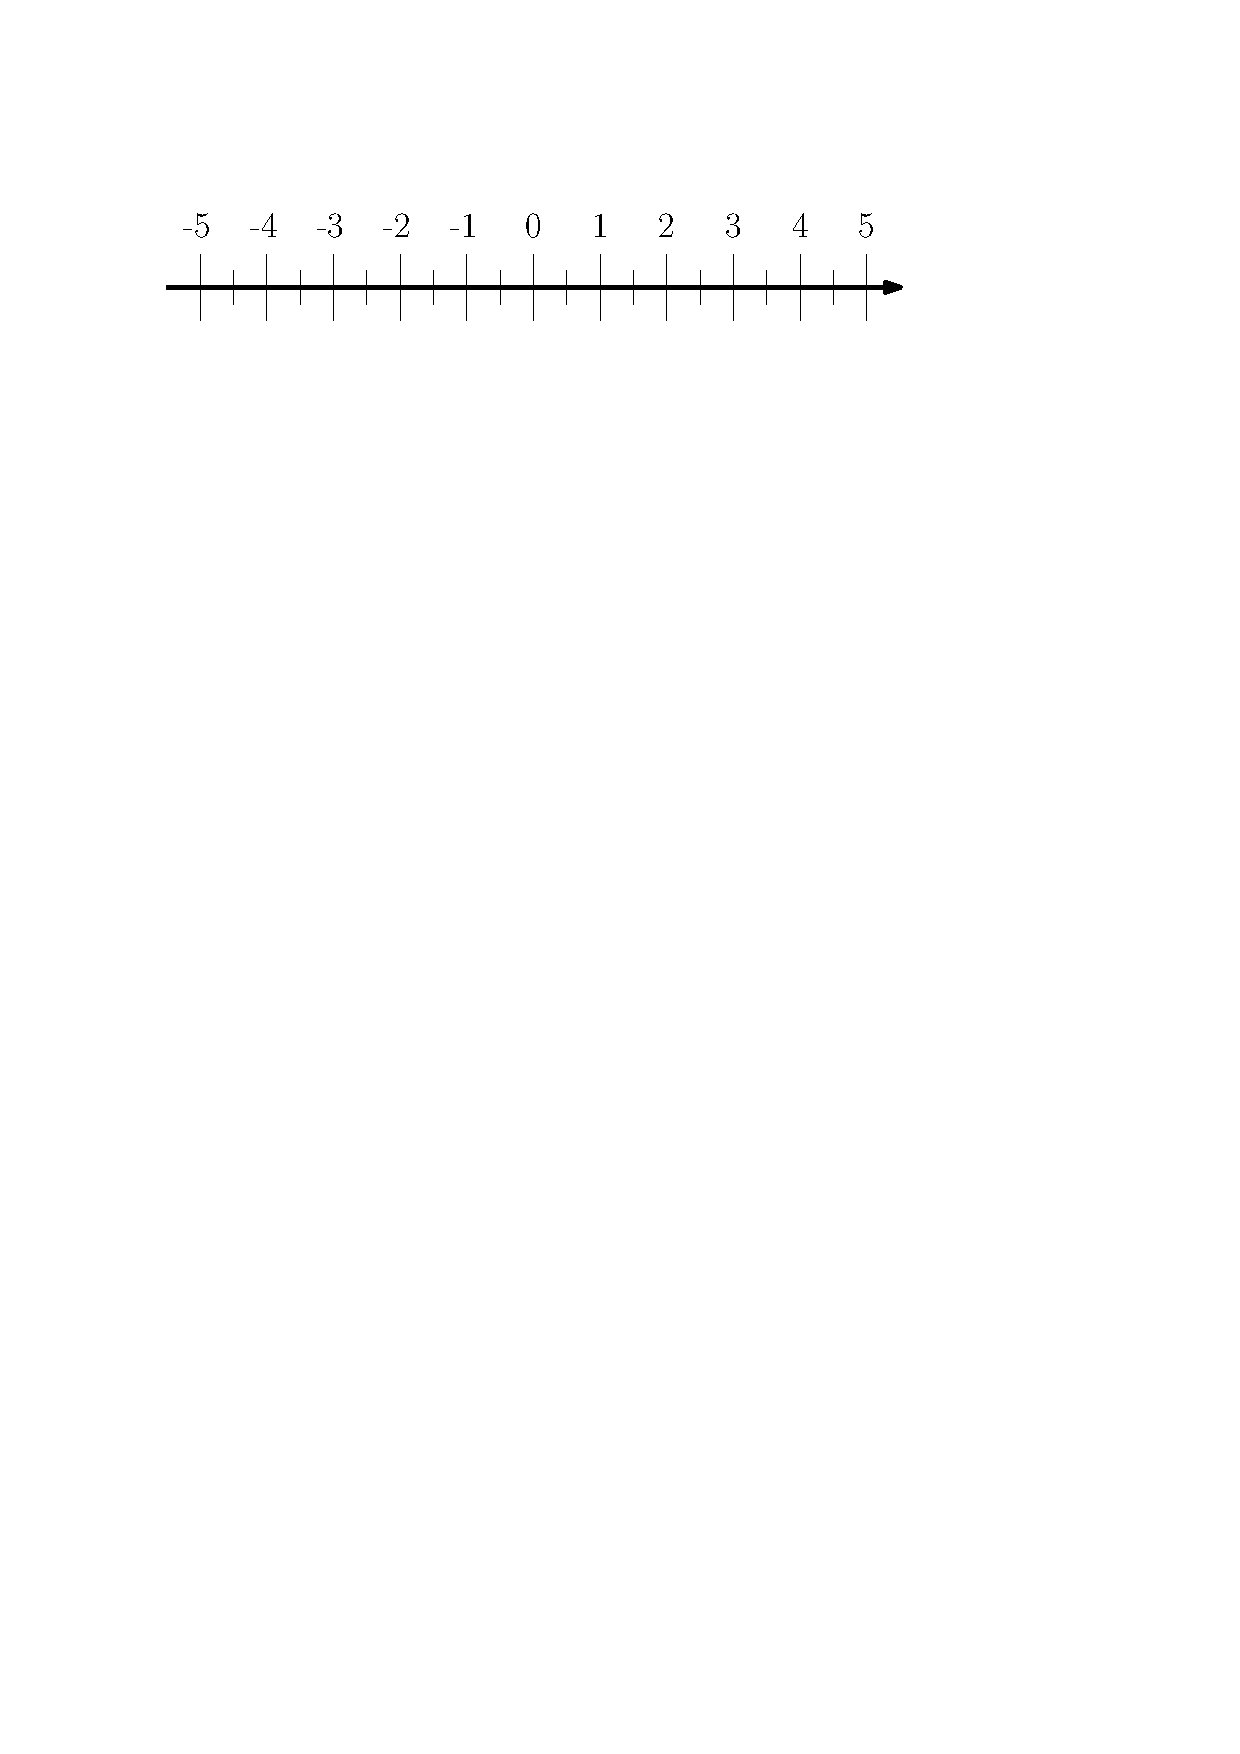
\includegraphics[width=0.9\linewidth]{5x4-relatifs/c-axe-1.pdf}
\end{figure}

$A = \SI{-2,5}{} ; B = \SI{2,25}{} ; C = \SI{-3,75}{} ; D = \SI{-3,8}{} ; E = \SI{-0,8}{}$

\begin{figure}[H]
  \centering
  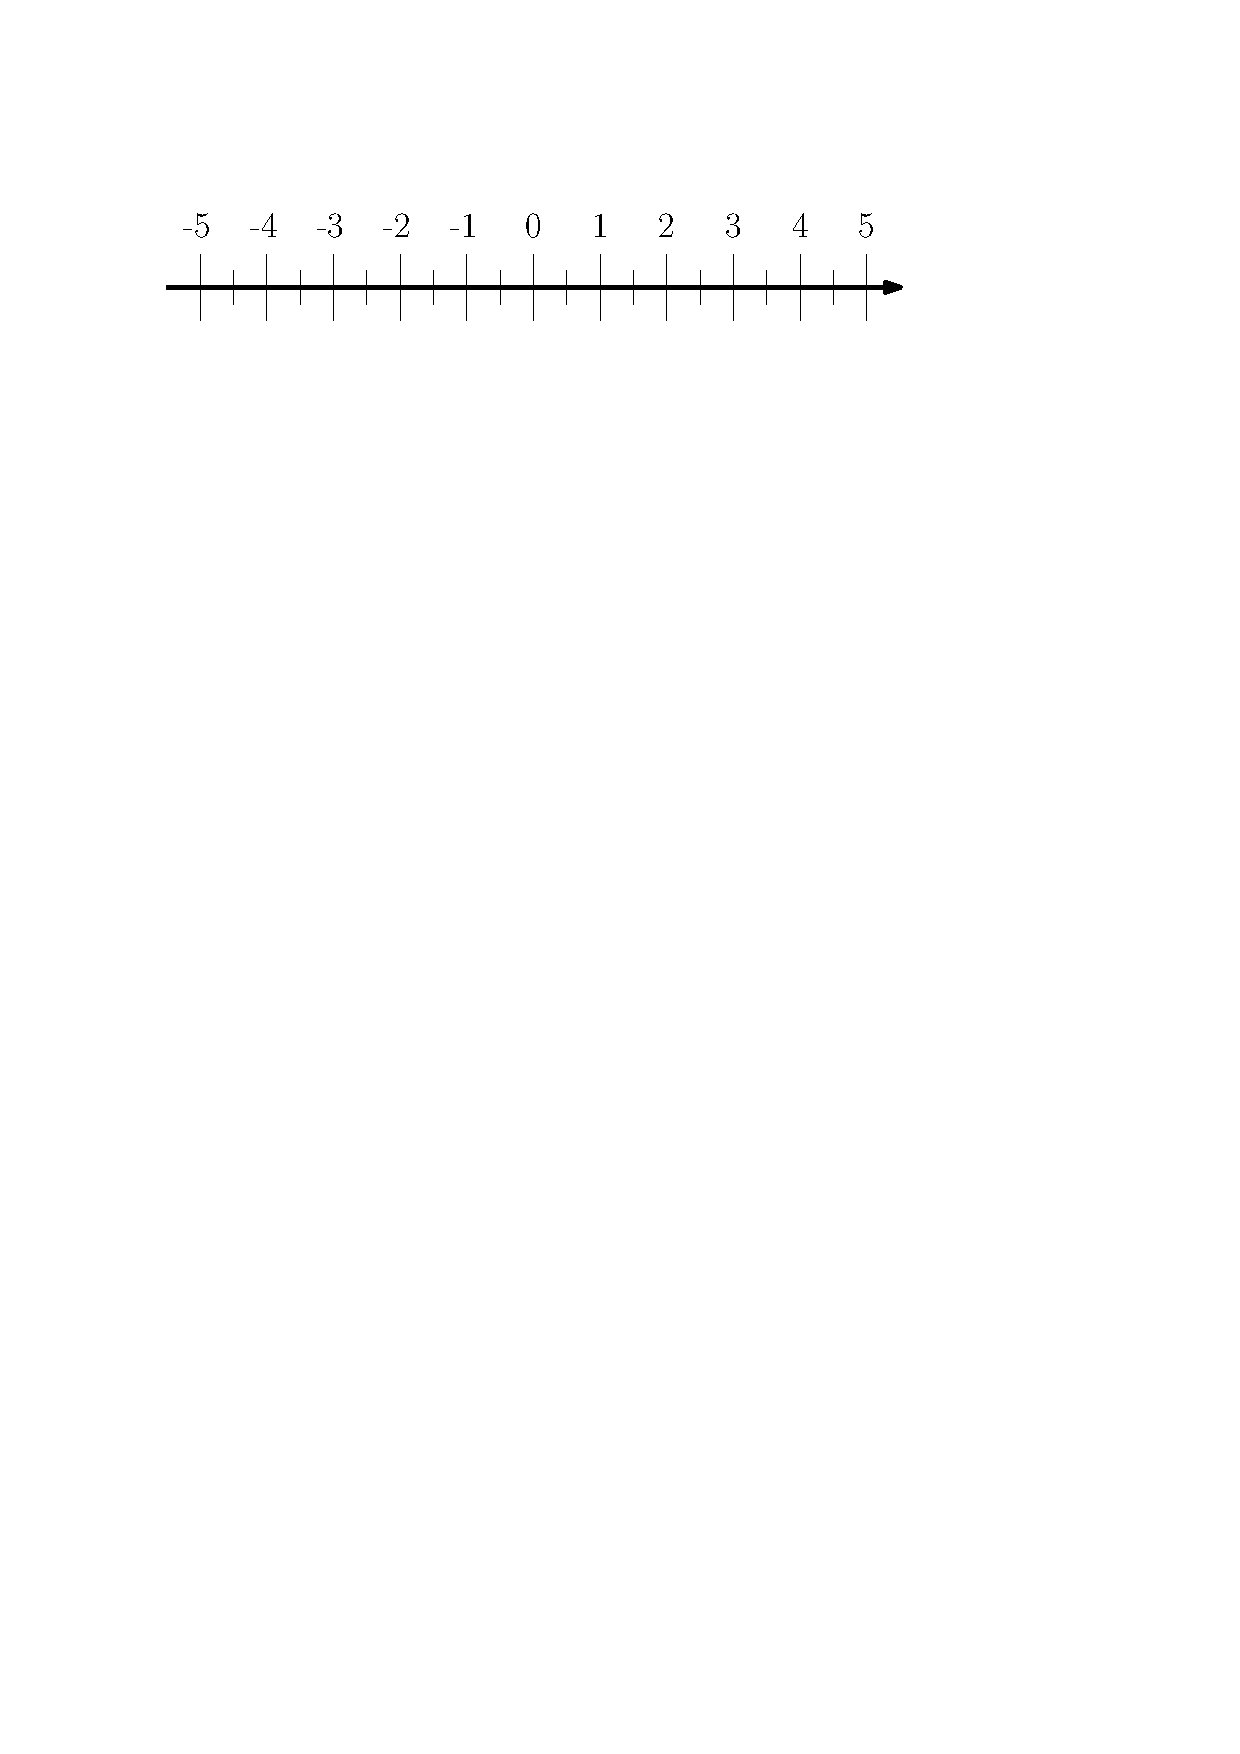
\includegraphics[width=0.9\linewidth]{5x4-relatifs/c-axe-1.pdf}
\end{figure}

\newpage


\textbf{Nom, Prénom :} \hspace{8cm} \textbf{Classe :} \hspace{3cm} \textbf{Date :}\\

\begin{center}
  \textit{La normalité est une route pavée : on y marche aisément mais les fleurs n’y poussent pas.}  - \textbf{Vincent Van Gogh}
\end{center}

\subsection*{Restituer les connaissances}

\begin{enumerate}
  \item[1.] Nombres négatifs : \dotfill \\
  \item[2.] Nombres opposés \dotfill \\
\end{enumerate}

\subsection*{Représenter des nombres par des opérations}

\begin{multicols}{2}

  \textit{Écrire le nombre négatif et l'opération correspondante.}

  \begin{enumerate}
    \item[1.] $  -7 = $ \dotfill
    \item[2.] $-120 = $ \dotfill
    \item[3.] $-0,8 = $ \dotfill
    \item[4.] $-\pi = $ \dotfill
    \item[5.] $ -\frac{1}{9} = $ \dotfill
    \item[6.] $0 - 15 = $  \dotfill
    \item[7.] $0 - \SI{2,45}{} = $  \dotfill
    \item[8.] $0 - \SI{33000}{} = $  \dotfill   
  \end{enumerate}
  \columnbreak

  \textit{Écrire l'opposé et l'opération correspondante.}

  \begin{enumerate}
    \item[1.] L'opposé de $8$ est \dots \dots car \dotfill
    \item[2.] L'opposé de $-5$ est \dots \dots car \dotfill
    \item[3.] L'opposé de $\SI{2500}{}$ est \dots \dots car \dotfill
    \item[4.] L'opposé de $\SI{-0,3}{}$ est \dots \dots car \dotfill
    \item[5.] L'opposé de $\pi$ est \dots \dots car \dotfill
    \item[6.] L'opposé de $\dfrac{2}{9}$ est \dots \dots car \dotfill
  \end{enumerate}

\end{multicols}

\subsection*{Comparer}

\textit{Ranger par ordre croissant. Utiliser le symbole $<$.}

\begin{enumerate}
  \item[1.] 0; 2; -4; 6; -8; -10
  \Pointilles[1]   
  \item[2.] 24; -21; \SI{2,6}{} ; \SI{-2,6}{} ; \SI{-2,5}{} , \SI{-2,55}{} 
  \Pointilles[1]   
  \item[3.] -200 ; 150 ; \SI{-34000}{} ; -50 ; 0,8 ; -90
  \Pointilles[1]   
\end{enumerate}

\subsection*{Droite graduée}

\textit{Placer les points sur la droite graduée.}

$A = -2 ; B = 3 ; C = \SI{-1,5}{} ; D = \SI{2,5}{} ; E = \SI{-0,5}{}$

\begin{figure}[H]
  \centering
  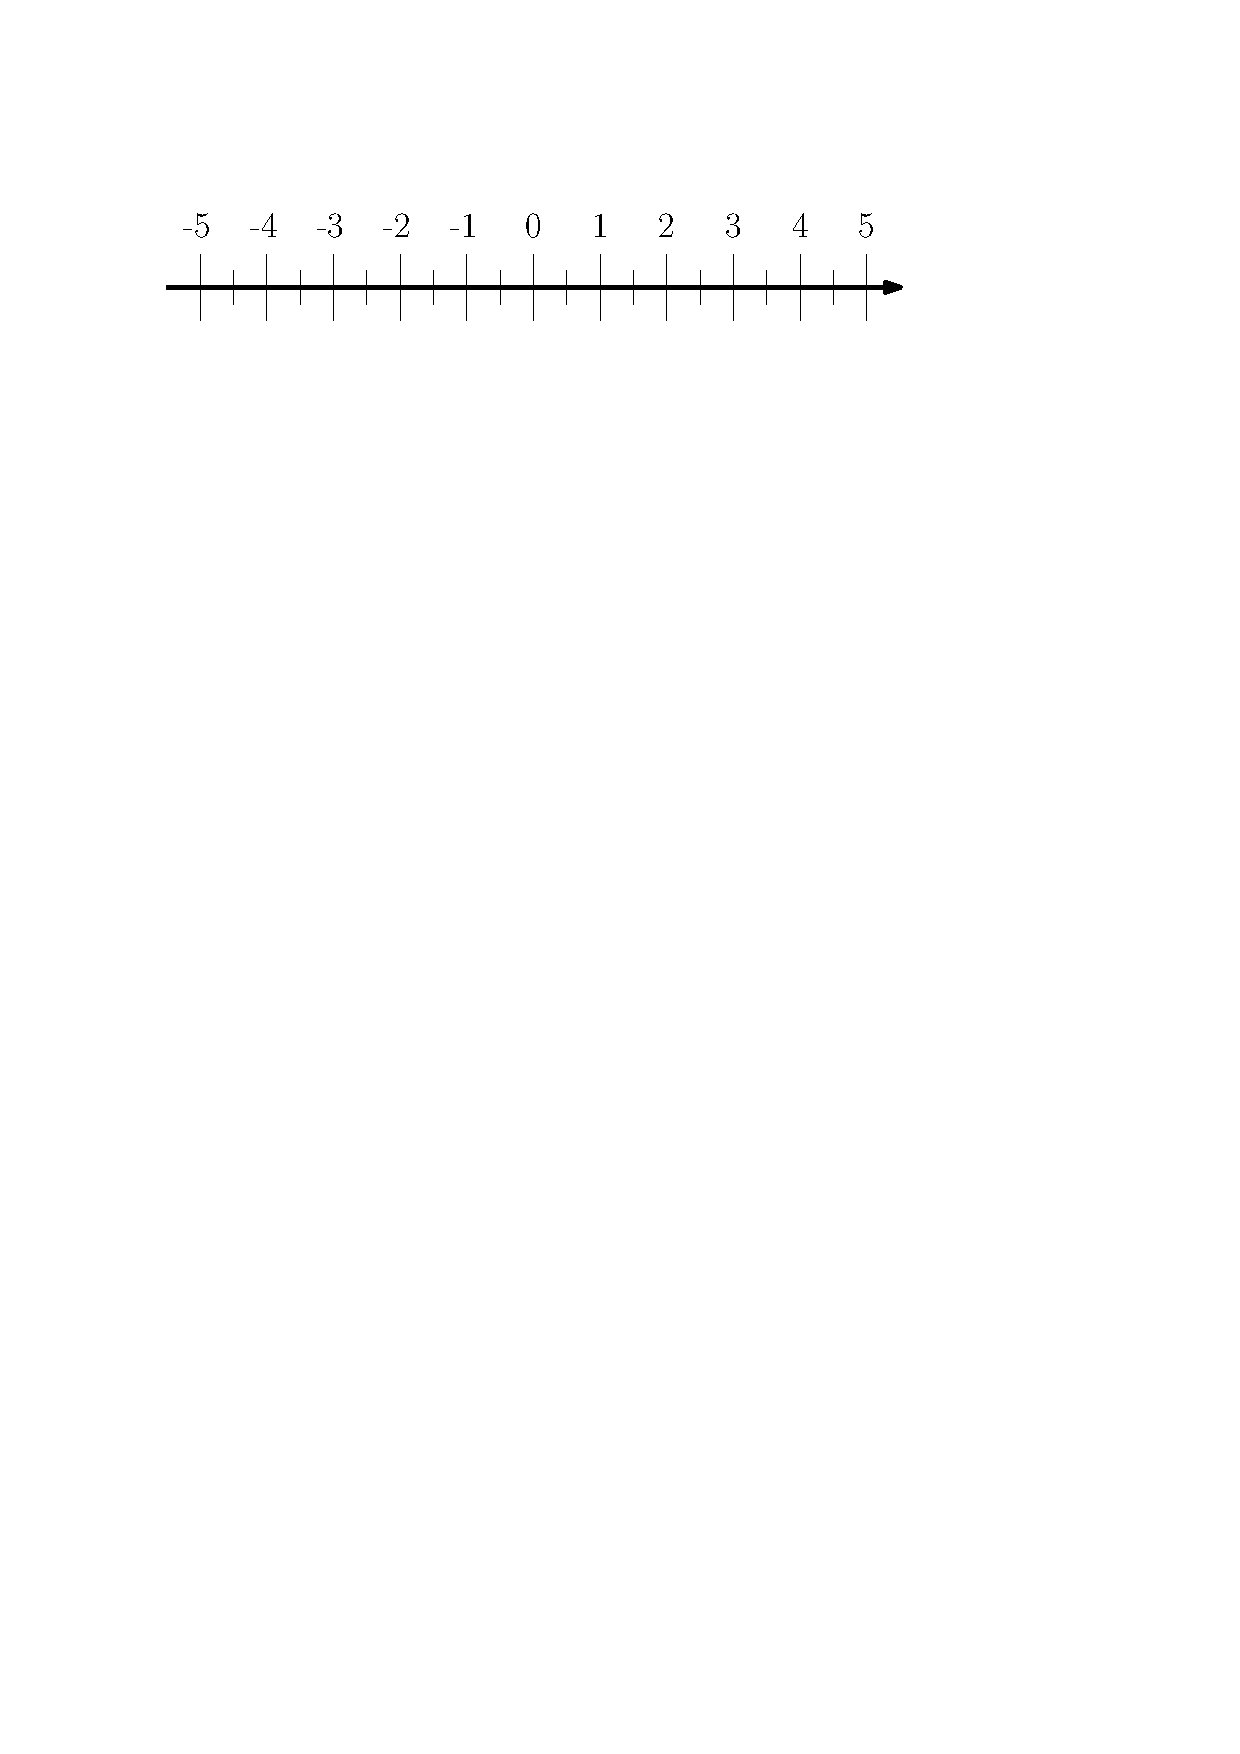
\includegraphics[width=0.9\linewidth]{5x4-relatifs/c-axe-1.pdf}
\end{figure}

$A = \SI{2,5}{} ; B = \SI{-2,25}{} ; C = \SI{3,75}{} ; D = \SI{-3,8}{} ; E = \SI{-0,4}{}$

\begin{figure}[H]
  \centering
  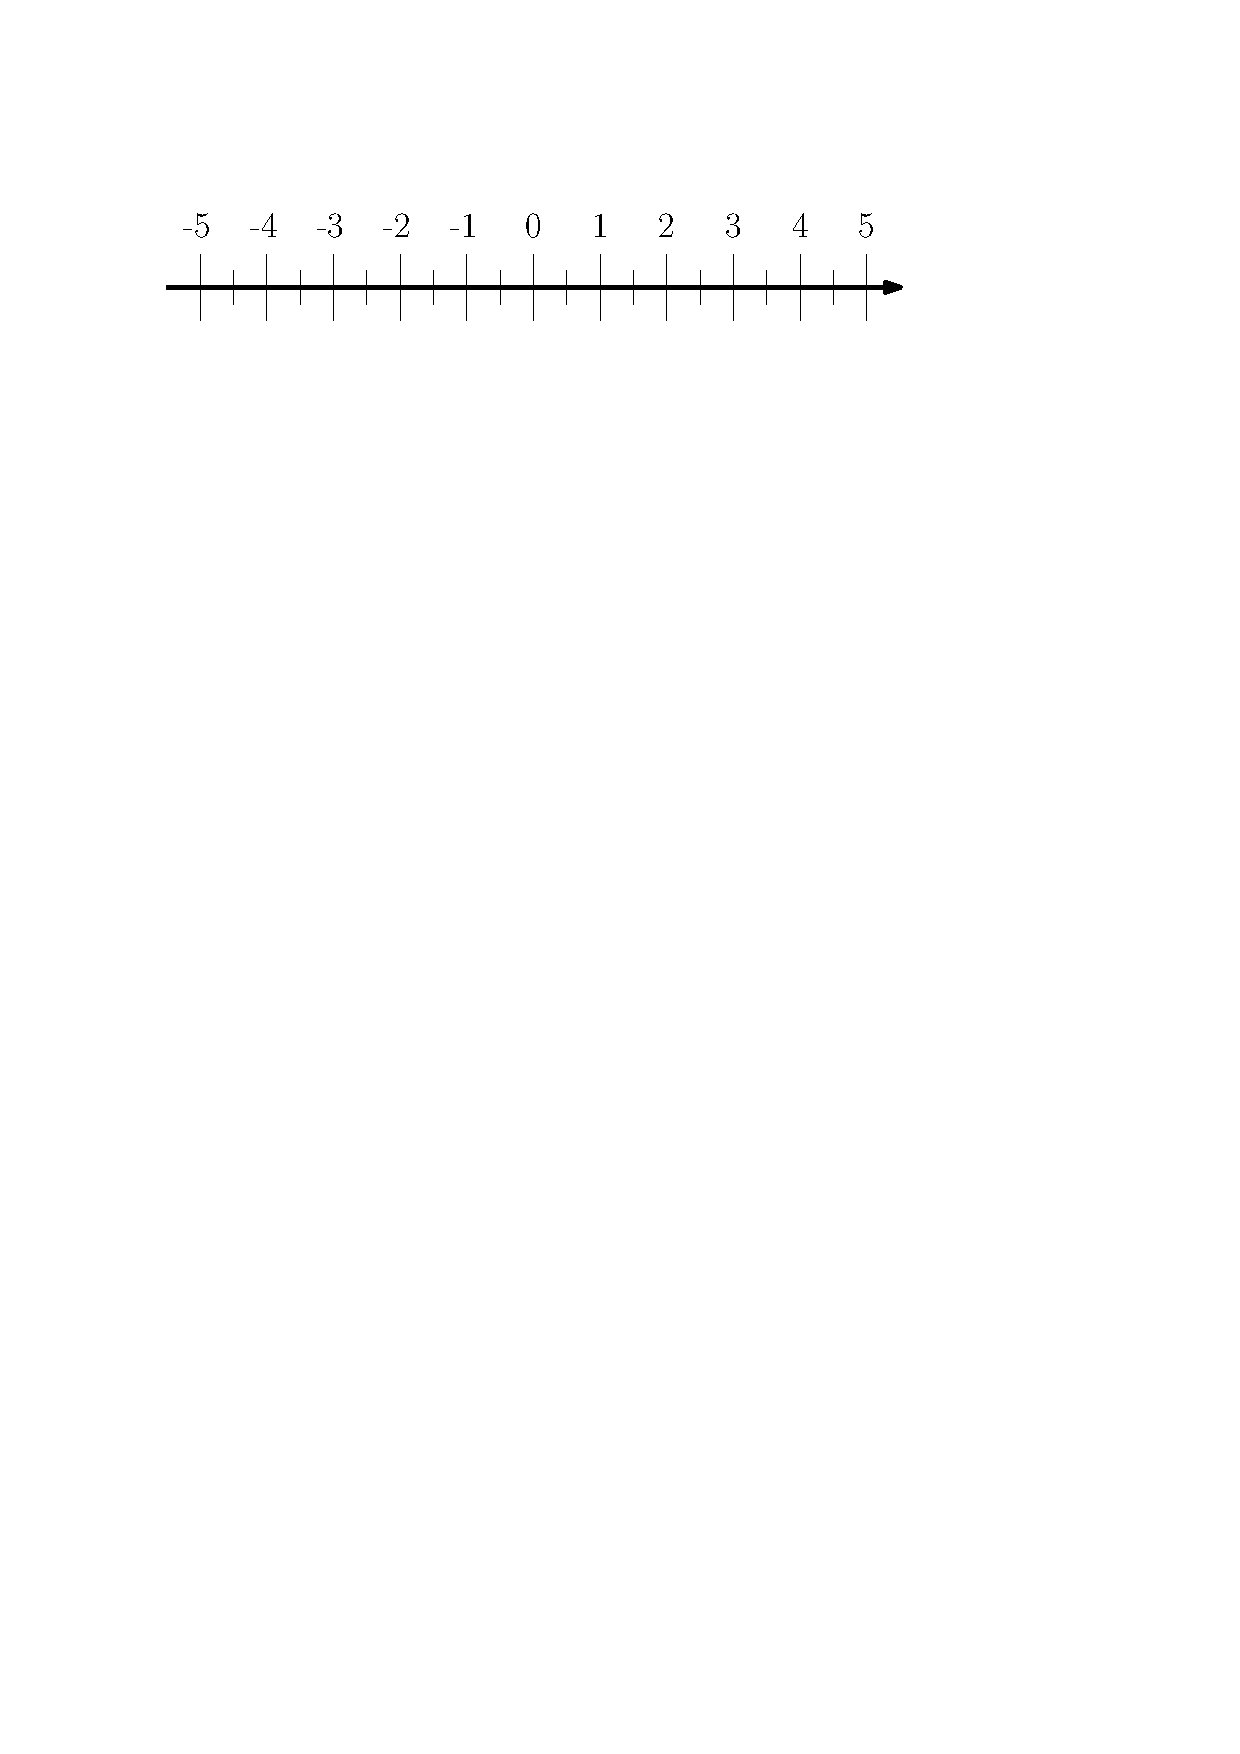
\includegraphics[width=0.9\linewidth]{5x4-relatifs/c-axe-1.pdf}
\end{figure}

\end{document}